\section{Evaluation \& Results}
\label{sec:evaluation}
We trained three model sizes (Table~\ref{tab:model-sizes}) and evaluate them on
standard ASR benchmarks and latency-sensitive streaming scenarios.

\begin{table*}[t]
    \centering
    \small
    \setlength{\tabcolsep}{4pt}
    \begin{tabular}{l c c c r r r r r}
    \toprule
    & \multicolumn{3}{c}{Architecture} & \multicolumn{5}{c}{Params (M)} \\
    \cmidrule(lr){2-4} \cmidrule(lr){5-9}
    Model & Enc dim & Dec dim & Layers (Enc/Dec) & Pre & Enc & Adap & Dec & Total \\
    \midrule
    Tiny   & 320 & 320 & 6/6   & 2.08 & 7.39 & 1.31 & 22.80 & 33.57 \\
    Small & 620 & 512 & 10/10 & 7.74 & 43.49 & 2.86 & 69.27 & 123.36 \\
    Medium & 768 & 640 & 14/14 & 11.86 & 93.66 & 3.64 & 135.77 & 244.93 \\
    \bottomrule
    \end{tabular}
    \caption{Moonshine v2 model architecture sizes and parameter breakdown by block.}
    \label{tab:model-sizes}
\end{table*}


\noindent\textbf{Note on parameter distribution.} The decoder has substantially more parameters than the encoder, largely because each decoder layer includes additional cross-attention projection matrices (in addition to self-attention), and because our decoder uses SwiGLU feed-forward blocks while the encoder does not.

\subsection{Experimental setup}
\subsubsection{Training.}
\paragraph{Data.} We use the same data sources and preprocessing pipeline as in the original
Moonshine work~\citep{jeffries2024moonshinespeechrecognitionlive} (see their
Section~3.2, \emph{Training data collection \& preprocessing}). Relative to that
setup (\,$\approx$200K hours total), we add an additional 100K hours of
internally prepared speech data, for a total of roughly 300K hours.

\paragraph{Tokenizer \& optimization. }We use the same tokenizer as in the original Moonshine
work~\citep{jeffries2024moonshinespeechrecognitionlive}. We also use the same
optimizer (Schedule-Free;~\citep{defazio2024roadscheduled}) with a starting
learning rate of $2\times10^{-3}$. Training was run for 400K steps with an
effective batch size of 512 on a cluster of 8 NVIDIA H100 GPUs.

\subsubsection{Implementation.}
We evaluate accuracy using the implementation in the Transformers
library~\citep{wolf2020transformers}. Note that this code path does not yet
perform fully efficient streaming; it relies on the flash-attention backend's
sliding-window attention when available. We measure latency separately
using our own library implementation of Moonshine in C++, which leverages the ONNX
runtime on CPU.~\footnote{https://github.com/moonshine-ai/moonshine}

\subsubsection{Benchmarks.}
We evalute the performance of Moonshine v2 using the following benchmarks.

\paragraph{Word error rate (WER).} We evaluate the WER of Moonshine v2 variants against similarly-sized models on the Open ASR leaderboard~\citep{srivastav2025open}.

\paragraph{Time-to-first-token (TTFT).} We empirically establish the latency differences between full and sliding window attention by comparing TTFT measurements of the original Moonshine~\citep{jeffries2024moonshinespeechrecognitionlive} full attention encoder to the Moonshine v2 sliding window encoder.

\paragraph{Response latency.} We perform empirical latency evaluations between Moonshine v2, the original Moonshine models, and the OpenAI Whisper models~\citep{radford2022robustspeechrecognitionlargescale} (as implemented in faster-whisper~\footnote{https://github.com/SYSTRAN/faster-whisper}). ASR models like Whisper were originally intended for offline processing scenarios, where the overall throughput of the system is important. Since our use case targets online processing applications (e.g., live captioning), we measure the real-time \emph{response latency} rather than throughput. We define this as the amount of time taken between detecting the end of a speech segment in an audio stream (via a voice activity detection (VAD) model) and the transcript text being returned. This is representative of, e.g,. the amount of time an embedded voice command system might take to detect a command after a typical utterance. We compare against Whisper because it has been adopted in embedded applications (via, e.g., whisper.cpp) despite its original design intent as an offline model, and against the original Moonshine models since they were designed for real-time use cases.

\paragraph{Compute cost.} We empirically measure compute cost by totalling the duration of the audio processing times for each model, and then expressing that as a percentage of the total audio duration. This is the inverse of the commonly used real-time factor (RTF) metric, but it reflects the compute load required for a real-time application.

We run empirical evaluations on an Apple M3.

\subsection{Results}
Table~\ref{tab:open-asr-results} reports WERs for individual datasets. We include it
for completeness, but the more informative view is the accuracy--parameter
tradeoff in Figure~\ref{fig:open-asr-avg-scatter}. That plot shows Pareto
frontiers in parameter count versus accuracy. The NVIDIA and Moonshine models
lie on a similar frontier and sit above OpenAI's. Moonshine fills the lower end
of the frontier (in parameter count), which is precisely the region we target:
efficient ASR models for 0.1--1 TOPs and memory-constrained edge processors
(e.g., sub-1~GB). NVIDIA's models, by contrast, are optimized for GPUs with tens
of GB of memory and multi-PFLOP compute.

% Table~\ref{tab:ttft-wer-comparison} reports TTFT, parameter count, and average WER on Open ASR 
% benchmarks for Moonshine v2 and Whisper models. Note that while Whisper models employ full attention
% in the encoder, they have a fixed TTFT since all inputs are padded to 30 seconds before encoding. 
% This table shows that Moonshine v2 models attain significantly lower fixed TTFT latency than Whisper models
% while achieving WER on par with significantly larger models. Moonshine v2 Medium, for instance, is 6x smaller than
% Whisper Large v3 but achieves effectively the same English transcription accuracy with 16x faster encoding.

Figure~\ref{fig:ttft-vs-moonshine} shows the differences in TTFT between full attention and sliding-window attention encoders by comparing the original Moonshine models with Moonshine v2. For longer utterances, even the largest Moonshine v2 achieves lower TTFT to the smaller Moonshine v1 models.

\begin{table}[t]
  \centering
  \small
  \begin{tabular}{l r r}
  \toprule
  Model & Latency (ms) & Compute Load (\%) \\
  \midrule
  \rowcolor{black!10} Moonshine Tiny & 27 & 5.91 \\
  \rowcolor{black!10} Moonshine Base & 44 & 7.34 \\
  \rowcolor{black!10} Moonshine v2 Tiny & 50 & 8.03 \\
  \rowcolor{black!10} Moonshine v2 Small & 148 & 17.97 \\
  \rowcolor{black!10} Moonshine v2 Medium & 258 & 28.95 \\
  Whisper Tiny & 289 & 8.46 \\
  Whisper Base & 553 & 16.19 \\
  Whisper Small & 1940 & 56.84 \\
  Whisper Large v3 & 11286 & 330.65 \\
  \bottomrule
  \end{tabular}
  \caption{Empirical response latency and compute load comparison for Moonshine and Whisper models. These values reflect the amount of time taken between the end of a speech utterance and the returned transcript in a real-time, live transcription scenario running on an Apple MacBook M3.}
  \label{tab:latency-comparison}
\end{table}

Table~\ref{tab:latency-comparison} compares the response latency between Moonshine, Moonshine v2, and Whisper models. The Moonshine v2 models demonstrate substantially lower latency than comparable Whisper models: Moonshine v2 Tiny achieves 50~ms latency (5.8x faster than Whisper Tiny), Moonshine v2 Small achieves 148~ms (13.1x faster than Whisper Small), and Moonshine v2 Medium achieves 258~ms (43.7x faster than Whisper Large v3), while also requiring less compute load on the same hardware.

\begin{table}[t]
  \centering
  \small
  \setlength{\tabcolsep}{6pt}
  \begin{tabular}{l r r r}
  \toprule
  Dataset & Tiny (34M) & Small (123M) & Med. (245M) \\
  \midrule
  AMI & 19.03 & 12.54 & 10.68 \\
  Earnings-22 & 20.27 & 13.53 & 11.90 \\
  GigaSpeech & 13.90 & 10.41 & 9.46 \\
  Libri (clean) & 4.49 & 2.49 & 2.08 \\
  Libri (other) & 12.09 & 6.78 & 5.00 \\
  SPGISpeech & 6.16 & 3.19 & 2.58 \\
  TED-LIUM & 6.12 & 3.77 & 2.99 \\
  VoxPopuli & 14.02 & 9.98 & 8.54 \\
  \midrule
  \textbf{Average} & \textbf{12.01} & \textbf{7.84} & \textbf{6.65} \\
  \bottomrule
  \end{tabular}
  \caption{WER (\%) for Moonshine v2 on Open ASR benchmarks.}
  \label{tab:open-asr-results}
\end{table}

\begin{figure*}[t]
  \centering
  \small
  \pgfplotstableread[col sep=comma]{
params,wer
2500,5.63
8000,5.74
2000,6.00
5600,6.02
600,6.05
600,6.32
1000,6.35
2600,6.40
1000,6.50
245,6.65
1550,6.67
1100,7.01
3000,7.05
1100,7.12
180,7.12
1000,7.15
756,7.21
1000,7.23
1100,7.40
1000,7.42
1000,7.43
1550,7.44
110,7.49
600,7.50
756,7.52
600,7.69
809,7.77
809,7.83
1550,7.83
123,7.84
756,7.92
1550,7.94
769,8.09
1000,8.12
1000,8.25
8000,8.52
166,8.57
244,8.59
394,8.77
61,9.99
74,10.32
19,10.61
34,12.01
27,12.65
39,12.81
} \openasravgall

  \pgfplotstableread[col sep=comma]{
params,wer,label
34,12.01,Moonshine v2 Tiny
123,7.84,Moonshine v2 Small
245,6.65,Moonshine v2 Medium
} \moonshinevTwo

  \pgfplotstableread[col sep=comma]{
params,wer
1550,7.44
809,7.83
1550,7.83
1550,7.94
769,8.09
244,8.59
74,10.32
39,12.81
} \openaiModels

  \pgfplotstableread[col sep=comma]{
params,wer
2500,5.63
600,6.05
600,6.32
1000,6.35
1000,6.50
1100,7.01
1100,7.12
180,7.12
1000,7.15
1100,7.40
110,7.49
600,7.50
600,7.69
} \nvidiaModels

  \pgfplotstableread[col sep=comma]{
params,acc
34,87.99
123,92.16
245,93.35
} \moonshineFrontier

  \pgfplotstableread[col sep=comma]{
params,acc
39,87.19
74,89.68
244,91.41
769,91.91
809,92.17
1550,92.56
} \openaiFrontier

  \pgfplotstableread[col sep=comma]{
params,acc
110,92.51
180,92.88
600,93.95
2500,94.37
} \nvidiaFrontier

  \begin{tikzpicture}
    \begin{axis}[
      width=\textwidth,
      height=0.45\textwidth,
      xmode=log,
      log basis x=10,
      xmin=10,
      xmax=10000,
      ymin=86,
      ymax=95,
      xlabel={Parameters (M, log scale)},
      ylabel={Accuracy (100 - WER, \%)},
      grid=both,
      major grid style={line width=0.2pt, draw=gray!30},
      minor grid style={line width=0.1pt, draw=gray!15},
      tick align=outside,
      tick style={line width=0.2pt},
      legend style={draw=none, font=\scriptsize, at={(0.02,0.98)}, anchor=north west},
      legend cell align=left,
    ]
      \addplot[
        only marks,
        mark=*,
        mark size=1.6pt,
        color=black!35
      ] table[x=params, y expr=100-\thisrow{wer}] {\openasravgall};
      \addlegendentry{Other models}

      \addplot[
        no marks,
        line width=0.8pt,
        color=msCyan
      ] table[x=params, y=acc] {\moonshineFrontier};

      \addplot[
        no marks,
        line width=0.8pt,
        color=msOrange
      ] table[x=params, y=acc] {\openaiFrontier};

      \addplot[
        no marks,
        line width=0.8pt,
        color=msGreen
      ] table[x=params, y=acc] {\nvidiaFrontier};

      \addplot[
        only marks,
        mark=*,
        mark size=2.6pt,
        color=msCyan,
        nodes near coords,
        point meta=explicit symbolic,
        every node near coord/.append style={font=\scriptsize, yshift=2pt, anchor=south, text=msCyan}
      ] table[x=params, y expr=100-\thisrow{wer}, meta=label] {\moonshinevTwo};
      \addlegendentry{Moonshine v2}

      \addplot[
        only marks,
        mark=triangle*,
        mark size=2.2pt,
        color=msOrange
      ] table[x=params, y expr=100-\thisrow{wer}] {\openaiModels};
      \addlegendentry{OpenAI}

      \addplot[
        only marks,
        mark=square*,
        mark size=2.2pt,
        color=msGreen
      ] table[x=params, y expr=100-\thisrow{wer}] {\nvidiaModels};
      \addlegendentry{NVIDIA}

      \addplot[
        only marks,
        mark=*,
        mark size=2.8pt,
        color=msGreen,
        nodes near coords,
        point meta=explicit symbolic,
        every node near coord/.append style={
          font=\scriptsize,
          anchor=west,
          xshift=2pt,
          text=msGreen
        }
      ] coordinates {(2500,94.37) [nvidia/canary-qwen-2.5b]};

      \addplot[
        only marks,
        mark=*,
        mark size=2.8pt,
        color=msGreen,
        nodes near coords,
        point meta=explicit symbolic,
        every node near coord/.append style={
          font=\scriptsize,
          anchor=west,
          xshift=5pt,
          yshift=1pt,
          text=msGreen
        }
      ] coordinates {(600,93.95) [nvidia/parakeet-tdt-0.6b-v2]};

      \addplot[
        only marks,
        mark=*,
        mark size=2.8pt,
        color=msOrange,
        nodes near coords,
        point meta=explicit symbolic,
        every node near coord/.append style={
          font=\scriptsize,
          anchor=west,
          xshift=2pt,
          text=msOrange
        }
      ] coordinates {(1550,92.56) [openai/whisper-large-v3]};

      \addplot[
        only marks,
        mark=*,
        mark size=2.8pt,
        color=msOrange,
        nodes near coords,
        point meta=explicit symbolic,
        every node near coord/.append style={
          font=\scriptsize,
          anchor=north east,
          xshift=-2pt,
          yshift=-1pt,
          text=msOrange
        }
      ] coordinates {(809,92.17) [openai/whisper-large-v3-turbo]};
    \end{axis}
  \end{tikzpicture}
  \vspace{-16pt}
  \caption{Accuracy vs. parameter count on Open ASR leaderboard averages.}
  \label{fig:open-asr-avg-scatter}
\end{figure*}


% \input{figures/tables/ttft_wer.tex}

\begin{figure}[t]
    \centering
    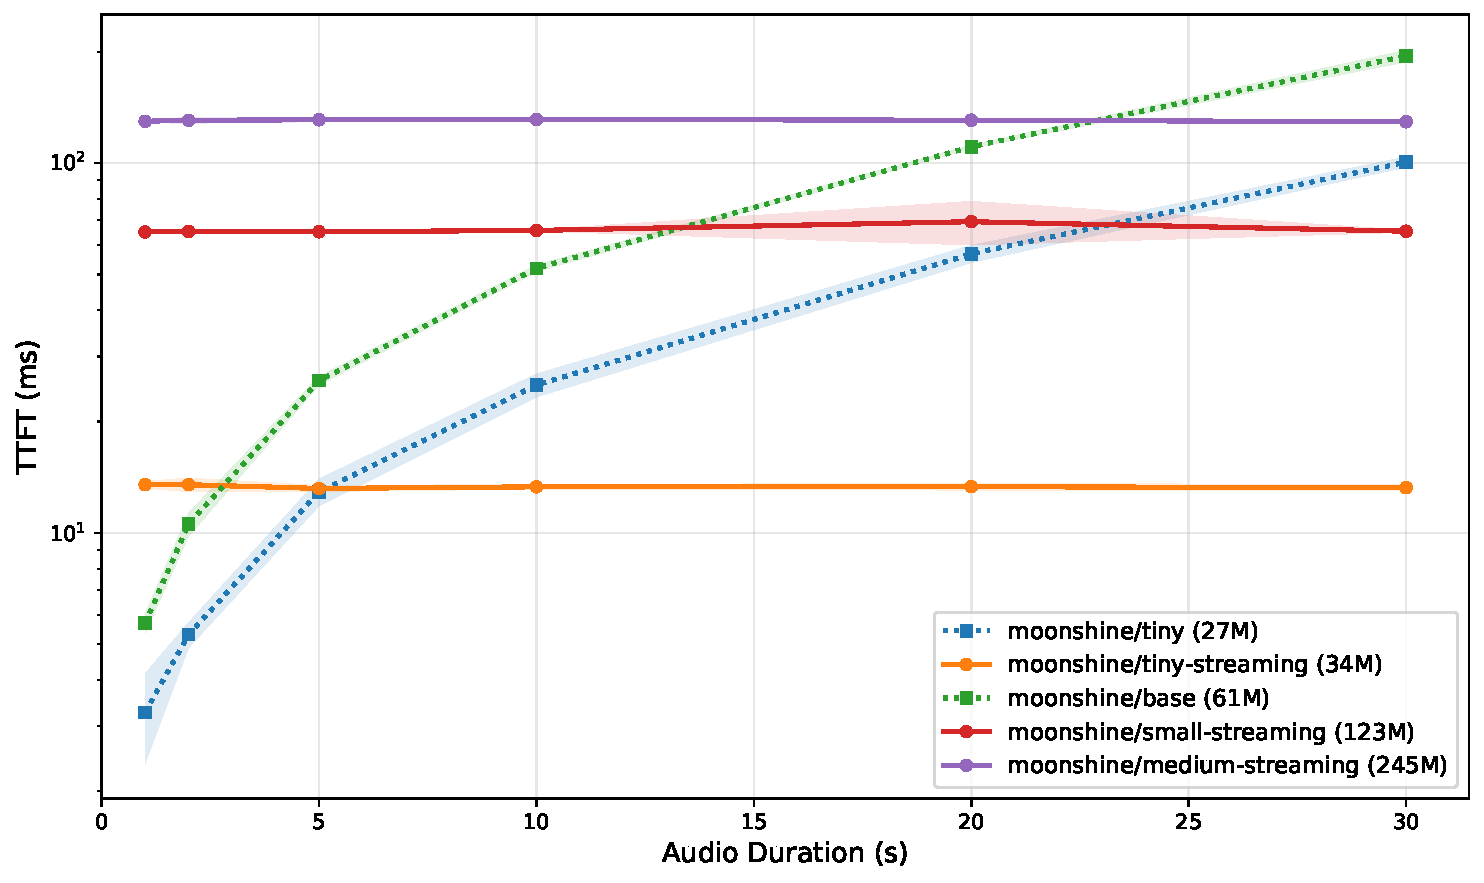
\includegraphics[width=\columnwidth]{figures/plots/ttft_moonshine.pdf}
    \caption{Time to first token (TTFT) versus input audio duration for Moonshine and Moonshine v2 models. The original Moonshine models use a full-attention encoder, which results in TTFT latency that grows with input audio duration. Sliding window attention in the Moonshine v2 encoder results in a fixed encoding latency, regardless of audio duration.}
    \label{fig:ttft-vs-moonshine}
\end{figure}
